\documentclass[11pt,a4paper,oneside]{report}

% --------------------------------------------------
% Packages
% --------------------------------------------------
\usepackage[T1]{fontenc}
\usepackage{lmodern}
\usepackage{amsmath}
\usepackage{amssymb}
\usepackage{graphicx}
\usepackage[a4paper,margin=1in]{geometry}
\usepackage{hyperref}
\usepackage{xcolor}
\usepackage{listings}
\usepackage{graphicx}
\usepackage{tikz}
\usetikzlibrary{positioning}

% --------------------------------------------------
% PDF metadata and hyperlinks
% --------------------------------------------------
\hypersetup{
    pdftitle={LearnDeep: Technical Reference},
    pdfauthor={Subhodeep Mondal},
    pdfsubject={Architecture and implementation of a deep learning framework},
    colorlinks=true,
    linkcolor=blue,
    urlcolor=blue,
    citecolor=blue
}

% --------------------------------------------------
% Cpp Language Setup
% --------------------------------------------------
% Custom color definitions for C++ syntax
\definecolor{mBackground}{rgb}{0.97,0.97,0.98}
\definecolor{mKeyword}{rgb}{0.0, 0.4, 0.65}
\definecolor{mString}{rgb}{0.13, 0.54, 0.13}
\definecolor{mComment}{rgb}{0.5, 0.5, 0.5}
\definecolor{mNumber}{rgb}{0.7, 0.2, 0.1}

% Global C++ style configuration
\lstdefinestyle{mycppstyle}{
    language=C++,
    backgroundcolor=\color{mBackground},
    commentstyle=\color{mComment}\itshape,
    keywordstyle=\color{mKeyword}\bfseries,
    numberstyle=\tiny\color{mComment},
    stringstyle=\color{mString},
    basicstyle=\ttfamily\small,
    breakatwhitespace=false,
    breaklines=true,
    captionpos=b,
    keepspaces=true,
    numbers=left,
    numbersep=8pt,
    showspaces=false,
    showstringspaces=false,
    showtabs=false,
    tabsize=4,
    frame=single,                     % Adds a border around the code
    rulecolor=\color{lightgray}       % Border color
}
\lstset{style=mycppstyle}

% --------------------------------------------------
% Document metadata
% --------------------------------------------------
\title{
    \textbf{LearnDeep}\\[0.5em]
    \large Technical Reference
}
\author{Subhodeep Mondal}
\date{\today}

% --------------------------------------------------
% Document
% --------------------------------------------------
\begin{document}

\maketitle

\pagenumbering{roman}
\tableofcontents
\clearpage

\pagenumbering{arabic}

% ==================================================
\chapter{Introduction}
% ==================================================

\section{Overview}

LearnDeep is an educational deep learning framework
developed from scratch to explore the fundamental
concepts, algorithms, and engineering principles
behind modern deep learning systems.

The primary objective of this project is to understand
how a deep learning framework operates internally,
from tensor computations and numerical kernels to
automatic differentiation, neural network layers,
and model training.

Rather than treating a deep learning framework as a
black box, LearnDeep aims to make its underlying
mechanisms explicit through a modular implementation
and a focus on mathematical correctness.

\section{Motivation}

Modern deep learning frameworks provide high-level
interfaces for constructing, training, and evaluating
neural networks. However, many of the mechanisms
responsible for these operations remain hidden behind
their public APIs.

Developing LearnDeep provides an opportunity to
investigate these mechanisms directly, including:

\begin{itemize}
    \item Tensor representation, indexing, and
          memory ownership.
    \item Numerical operations, broadcasting, and
          CPU and GPU kernel execution.
    \item Computational graphs and reverse-mode
          automatic differentiation.
    \item Neural network layers, loss functions,
          and gradient propagation.
    \item Model training, optimization, and execution
          management.
\end{itemize}

Implementing these components from the ground up
provides practical insight into the relationship
between mathematical operations, software
architecture, and hardware-level computation.

\section{Scope}

LearnDeep is intended primarily as a learning and
experimentation platform. Its implementation
prioritizes understanding, modularity, and correctness
while exploring the design of a deep learning framework.

The technical reference documents the framework's
architecture, public interfaces, mathematical
foundations, and important implementation decisions.

It is organized around the major components of the
system, allowing readers to understand both how
individual components work and how they interact
during model execution and training.

\section{Organization of This Document}

The remainder of this document is organized as follows:

\begin{itemize}
    \item \textbf{Tensor System:} Tensor representation,
          shape semantics, data layout, and ownership.
    \item \textbf{Operations and Kernels:} Numerical
          operations, broadcasting, and backend execution.
    \item \textbf{Automatic Differentiation:}
          Computational graphs, gradient propagation,
          and backward execution.
    \item \textbf{Neural Network Components:} Layers,
          loss functions, and model construction.
    \item \textbf{Training:} Forward execution,
          optimization, and training workflows.
\end{itemize}

These sections describe the design and behavior of
the implemented system, including relevant
mathematical definitions and validation methods.

\chapter{Deep Learning Framework from Scratch}
\label{chap:deep-learning-framework-from-scratch}


\section{Tensor 101}

A tensor is a multidimensional array. Scalars contain a single value, vectors extend this idea to one dimension, and matrices extend it to two dimensions. Tensors generalize the same concept to an arbitrary number of dimensions.

Einstein did not invent tensors, but his work helped popSularize their use in physics.

\subsection{Why Do We Need Tensors?}

To do mathematics, of course.

At a basic level, a tensor implementation needs a block of memory to store its elements and metadata describing the size of each dimension. In this implementation, the elements are stored in a contiguous memory allocation, while the dimensions are represented separately.

A simplified version of the class looks like this:

\begin{lstlisting}[
    language=C++,
    caption={A simplified tensor class},
    label={lst:basic-tensor-class}
]
template<typename T>
class tensor {
    T* data;                 // Manual memory management.
    size_t no_of_dimensions;
    size_t* dimensions;

public:
    tensor();
    ~tensor();

    tensor add(tensor b);
    tensor matmul(tensor b);
};
\end{lstlisting}

No \texttt{std::unique\_ptr}, no \texttt{std::vector}. As the joke goes: \emph{``Hum toh mard hai, Jaskirat. We manage our own memory.''}

Of course, manual memory management also means that allocation, deallocation, copying, and ownership must be handled carefully. This is one of the engineering trade-offs involved in building the underlying storage abstraction yourself.

For example,

\begin{lstlisting}[language=C++, caption={Creating a three-dimensional tensor}]
tf::tensor A(2, 3, 4);
\end{lstlisting}

creates a three-dimensional tensor with dimensions \((2,3,4)\). It contains 2 elements along the first dimension, 3 along the second, and 4 along the third, for a total of \(2 \times 3 \times 4 = 24\) elements.

Simple enough. No rocket science.

\subsection{A Different Dimension Convention}

There is an important design choice in LearnDeep: its dimension ordering differs from the convention commonly encountered in NumPy, TensorFlow, and PyTorch.

In LearnDeep, the leftmost dimension is treated as the primary dimension. Consequently, a tensor described by dimensions \((2,3,4)\) follows the framework's own axis convention and should not be assumed to have the same interpretation as a tensor with that shape in another library.

When comparing shapes or transferring data between frameworks, this difference must be taken into account. Changing the convention later would require careful refactoring of operations, kernels, and code that depends on the current layout.

For now, this is the convention used by LearnDeep.

\section{Working with Tensors}

Having a tensor abstraction is useful only if we can perform computations with it. Tensor operations provide the basic mathematical building blocks used throughout the framework.

For example, two tensors can be created, populated with data, and added together:

\begin{lstlisting}[
    language=C++,
    caption={Adding two tensors},
    label={lst:tensor-add-example}
]
tf::tensor A, B, C;

A.tf_create(2, 3, 4);
B.tf_create(2, 3, 4);

A.tensor_of(data_1);
B.tensor_of(data_2);

C = A.add(B);
\end{lstlisting}

Matrix multiplication can be expressed in a similar way:

\begin{lstlisting}[
    language=C++,
    caption={Matrix multiplication using LearnDeep's dimension convention},
    label={lst:tensor-matmul-example}
]
A.tf_create(2, 3);
B.tf_create(4, 2);

C = A.matmul(B);

// Result dimensions: (4, 3)
\end{lstlisting}

The result dimensions shown above follow LearnDeep's custom axis convention. They differ from the shape notation readers may expect when working with NumPy, so the framework's own conventions must be kept in mind when interpreting the operation.

These examples illustrate the public interface. The actual arithmetic is performed by the underlying operation and kernel implementation.

\section{How Should the Mathematics Be Implemented?}

BLAS, BLIS, LAPACK, cuBLAS, Eigen\ldots

Those libraries provide powerful implementations of numerical operations. However, the purpose of this project is to understand how such computations work internally, so I decided to implement the kernels myself.

One possible approach would be to place the implementation of every operation directly inside the tensor class:

\begin{lstlisting}[
    language=C++,
    caption={A direct implementation inside the tensor class},
    label={lst:tensor-inline-operation}
]
class tensor {
    tensor add(tensor input_b) {
        tensor output;

        // Iterate over the elements and add them.

        return output;
    }
};
\end{lstlisting}

This is simple to understand, but it mixes tensor storage and interface responsibilities with the implementation of individual operations.

Instead, LearnDeep separates operations from the tensor abstraction. This provides a place to organize computation and, as the framework grows, to support features such as:

\begin{enumerate}
    \item \textbf{Kernel dispatching:} selecting an appropriate implementation, such as a basic CPU, AVX2, or GPU kernel.
    \item \textbf{Kernel registration:} organizing the available kernel implementations.
    \item \textbf{Automatic differentiation:} associating operations with the information needed to calculate gradients during backpropagation.
\end{enumerate}

A simplified illustration of this idea is shown below:

\begin{lstlisting}[
    language=C++,
    caption={An illustrative abstraction for operations},
    label={lst:operation-abstraction}
]
class ops {
public:
    virtual void compute() = 0;
    virtual void kernel_dispatcher() = 0;
};

class add : protected ops {
public:
    void compute() override;
    void kernel_dispatcher() override;
};
\end{lstlisting}

This is a conceptual example rather than a complete representation of the final implementation. The design can evolve as additional operations and execution backends are introduced.

The important idea is to keep the tensor abstraction, operation definitions, and kernel execution strategy sufficiently separate. This gives the framework room to grow without forcing every new implementation detail into the tensor class itself.

\section{Testing and Numerical Verification}

Once the basic abstractions and operations are in place, the next step is testing.

For this project, NumPy serves as an independent numerical reference. I generate test data, calculate expected results using NumPy, and compare those results against the output produced by LearnDeep.

This approach helps identify discrepancies in tensor operations and provides a practical way to verify that the framework's computations behave as expected.

The tests are an important part of the development process: successful compilation alone does not establish that an operation is numerically correct.

% Replace the placeholders below with screenshots of the actual test suite
% and validation results. Keep the image files in the project image directory.
%
% \begin{figure}[htbp]
%     \centering
%     \includegraphics[width=\textwidth]{../images/tensor-test-results.png}
%     \caption{Tensor operation tests and numerical validation results.}
%     \label{fig:tensor-test-results}
% \end{figure}

\section{Closing Remarks}

This is the starting point of LearnDeep: a tensor abstraction, a growing set of mathematical operations, and an implementation strategy that leaves room for multiple kernel backends and automatic differentiation.

The framework will become more capable as these foundations are extended and connected. For now, the priority is to build the core carefully, test it against independent reference results, and understand the engineering decisions behind each component.

There is plenty left to do.

To be continued\ldots
\chapter{Operations}


\begin{figure}[!ht]
    \centering
    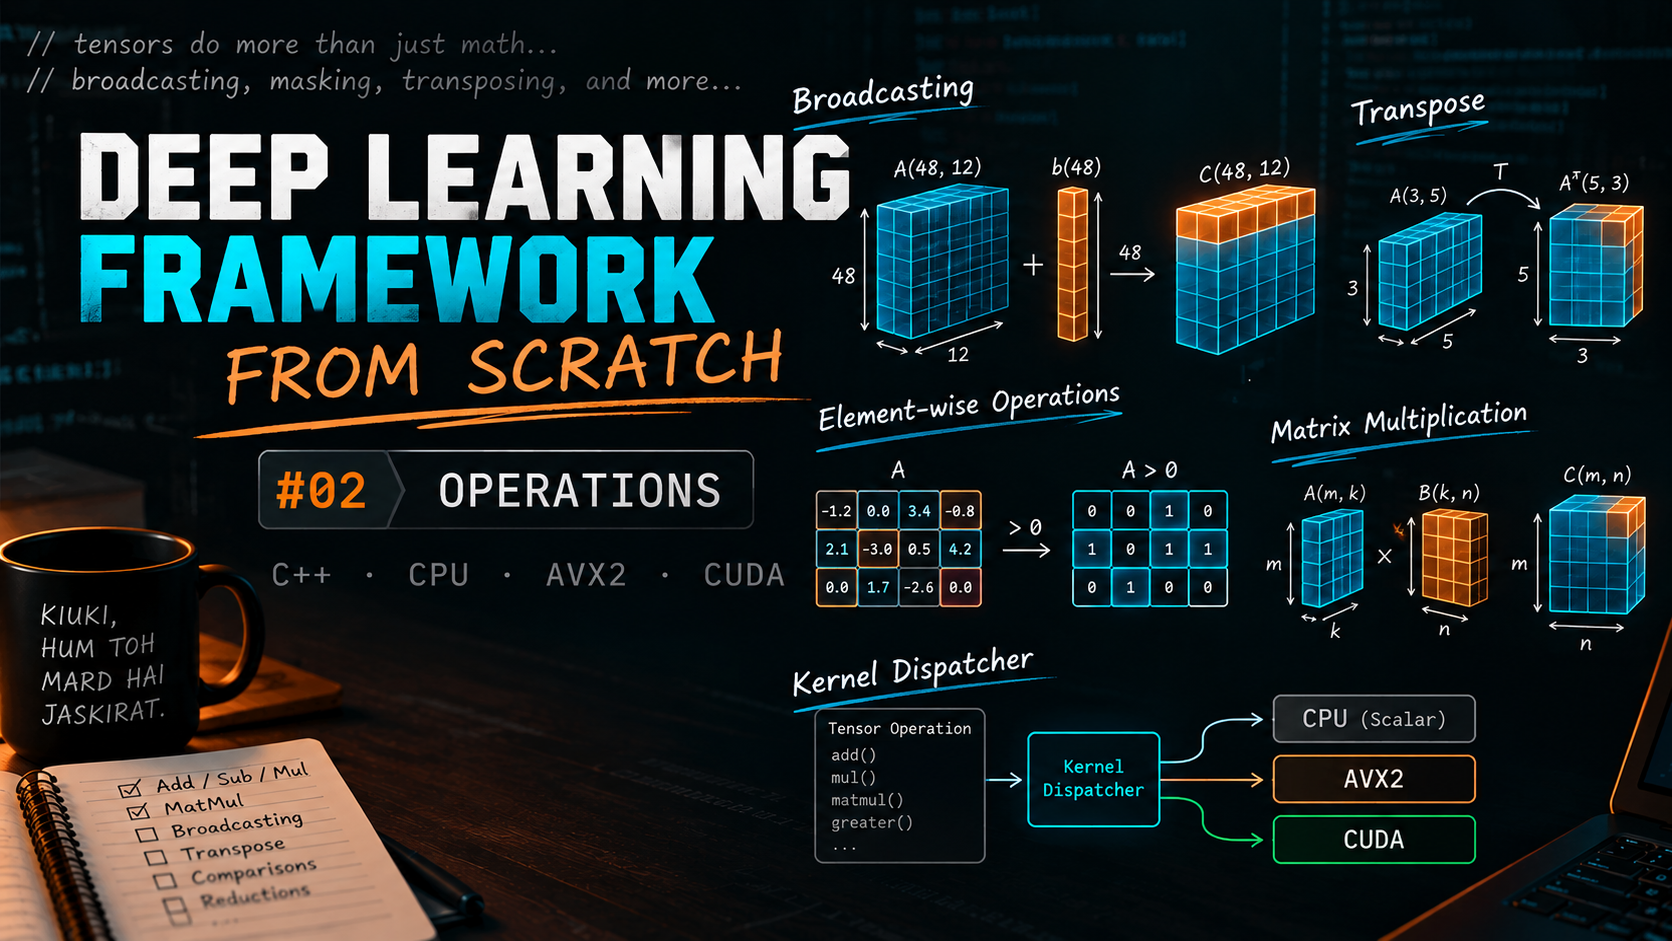
\includegraphics[width=\textwidth]{../../images/03_Tensor Operations From Scratch.png}
\end{figure}
\chapter{Kernels}
\chapter{Automatic Differentiation}
\label{chap:autograd}


\begin{figure}[!ht]
    \centering
    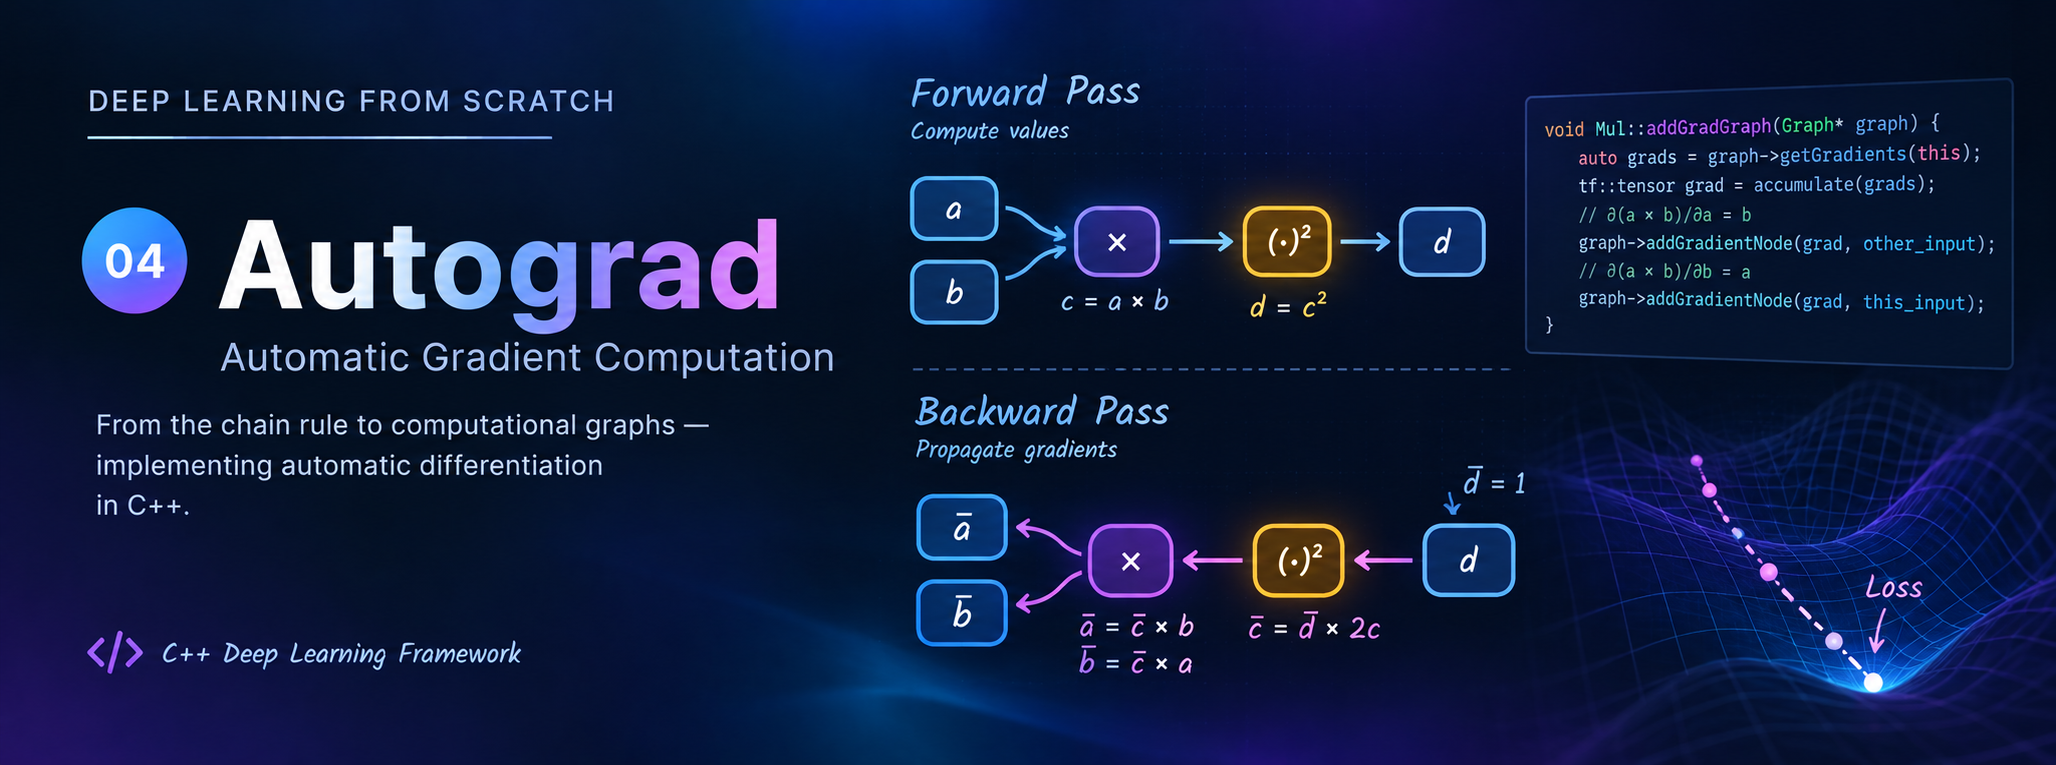
\includegraphics[width=\textwidth]{../../images/05_Autograd_ Forward and Backward Passes.png}
\end{figure}


\section{Autograd 101}

Automatic gradient computation, commonly called \emph{automatic differentiation} or \emph{autodiff}, is a technique for calculating derivatives of a computation with respect to its inputs and parameters.

Consider the function

\[
y = x^2 + 3x.
\]

Its derivative with respect to \(x\) is

\[
\frac{dy}{dx} = 2x + 3.
\]

For a simple expression, deriving the derivative manually is straightforward. However, neural networks can contain many tensor operations distributed across multiple layers. Manually deriving and implementing every possible derivative for every possible model would quickly become impractical.

Automatic differentiation addresses this problem by applying derivative rules to the operations performed during a computation and combining them using the chain rule.

It is important to distinguish autodiff from symbolic differentiation and numerical differentiation. Symbolic differentiation manipulates mathematical expressions to produce derivative expressions, while numerical differentiation estimates derivatives using numerical approximations, such as finite differences. Automatic differentiation instead propagates derivative information through the computation itself.

\section{Forward Propagation and Backward Propagation}

Consider a small example:

\[
a = 2,\qquad b = 3,
\]
\[
c = a+b,\qquad d = c^2.
\]

During the forward pass, the intermediate and final values are calculated:

\[
c = 5,\qquad d = 25.
\]

Suppose we want to calculate the derivatives of \(d\) with respect to \(a\) and \(b\). Applying the chain rule gives

\[
\frac{\partial d}{\partial c} = 2c = 10.
\]

Since \(c=a+b\),

\[
\frac{\partial c}{\partial a}=1,
\qquad
\frac{\partial c}{\partial b}=1.
\]

Therefore,

\[
\frac{\partial d}{\partial a}=10,
\qquad
\frac{\partial d}{\partial b}=10.
\]

The forward pass calculates the values of the computation, while the backward pass calculates how changes in those values influence the selected output.

This distinction is fundamental to training neural networks: the forward pass produces predictions and the backward pass computes the gradients needed to update trainable parameters.

\section{Why Reverse-Mode Automatic Differentiation?}

Automatic differentiation can be performed in different modes. Two commonly discussed approaches are forward-mode and reverse-mode differentiation.

\begin{itemize}
    \item \textbf{Forward mode} propagates derivative information alongside the forward computation.
    \item \textbf{Reverse mode} first evaluates the computation and then propagates gradients backward from the output.
\end{itemize}

Reverse mode is especially useful when a function has many inputs but relatively few outputs. Neural networks often have a large number of trainable parameters and a scalar loss, making reverse-mode differentiation a natural choice for computing the gradients required during training.

LearnDeep builds on its graph-mode execution to support this process. Since the forward operations and their dependencies are recorded in a computational graph, the framework can traverse those dependencies in reverse order and construct the corresponding gradient computation.

\section{Constructing the Gradient Graph}

The autodiff implementation in LearnDeep follows three broad steps:

\begin{enumerate}
    \item \textbf{Recording dependencies:} operations establish relationships between their input and output tensors in the computational graph.
    \item \textbf{Propagating gradients:} starting from the selected output, the framework visits operations in reverse dependency order and applies the derivative rule associated with each operation.
    \item \textbf{Accumulating gradients:} when a tensor contributes to multiple downstream operations, the gradient contributions from those paths must be added together.
\end{enumerate}

Each operation is responsible for registering the backward computation corresponding to its derivative rule. In LearnDeep, this responsibility is represented by an \texttt{addGradGraph()} routine that receives a pointer to the gradient graph.

The following simplified pseudocode illustrates the idea for a multiplication operation:

\begin{lstlisting}[
    language=C++,
    caption={Conceptual gradient-graph construction for multiplication},
    label={lst:mul-add-grad-graph}
]
void Mul::addGradGraph(Graph* graph) {
    // Retrieve gradients arriving from downstream operations.
    std::vector<tf::tensor> incoming_gradients =
        graph->getGradients(this);

    // Accumulate incoming gradients where necessary.
    // ...

    // For z = a * b:
    // dz/da = b
    // dz/db = a

    // Register backward operations that multiply the
    // incoming gradient by the opposite input.
    // ...

    // Store the resulting gradient nodes for each input.
}
\end{lstlisting}

The example is intentionally simplified. It illustrates the responsibilities of the routine rather than specifying the complete implementation or its ownership details.

For a multiplication \(z=ab\), the local derivatives are

\[
\frac{\partial z}{\partial a}=b,
\qquad
\frac{\partial z}{\partial b}=a.
\]

If the incoming gradient from downstream computation is \(\bar{z}\), the gradients propagated to the inputs are

\[
\bar{a}=\bar{z}b,
\qquad
\bar{b}=\bar{z}a.
\]

Here, the bar notation represents the gradient propagated to a tensor. In a computational graph with multiple downstream paths, these contributions must be accumulated before the gradient is propagated further upstream.

This is how the framework builds the backward computation associated with each supported operation.

\section{Visualizing the Forward and Backward Graphs}

Consider the computation

\[
c = a b,
\qquad
d = c^2.
\]

The forward graph describes how the output is calculated from the inputs:

\begin{center}
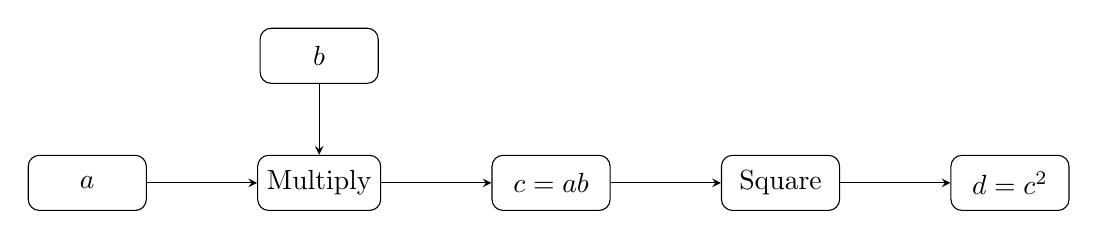
\begin{tikzpicture}[
    node distance=1.5cm,
    every node/.style={draw, rounded corners, align=center, minimum width=1.5cm, minimum height=0.7cm},
    >=stealth
]
\node (a) {\(a\)};
\node[right=1.4cm of a] (mul) {Multiply};
\node[above=0.9cm of mul] (b) {\(b\)};
\node[right=1.4cm of mul] (c) {\(c=ab\)};
\node[right=1.4cm of c] (sq) {Square};
\node[right=1.4cm of sq] (d) {\(d=c^2\)};
\draw[->] (a) -- (mul);
\draw[->] (b) -- (mul);
\draw[->] (mul) -- (c);
\draw[->] (c) -- (sq);
\draw[->] (sq) -- (d);
\end{tikzpicture}
\end{center}

The graph begins with the inputs \(a\) and \(b\). Multiplication produces \(c\), which is then squared to produce \(d\).

For reverse-mode differentiation, we seed the output gradient with

\[
\bar{d}=\frac{\partial d}{\partial d}=1.
\]

For the square operation,

\[
\bar{c}=\bar{d}\,2c.
\]

For the multiplication operation,

\[
\bar{a}=\bar{c}b,
\qquad
\bar{b}=\bar{c}a.
\]

The backward computation therefore follows the derivative rules of the forward operations, rather than simply repeating the original operations in reverse order.

\begin{center}
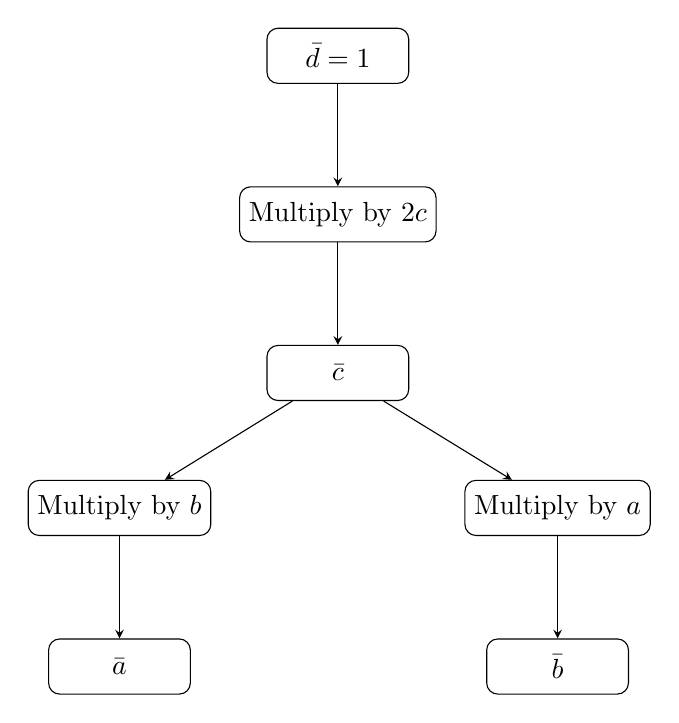
\begin{tikzpicture}[
    node distance=1.3cm,
    every node/.style={draw, rounded corners, align=center, minimum width=1.8cm, minimum height=0.7cm},
    >=stealth
]
\node (gd) {\(\bar{d}=1\)};
\node[below=of gd] (sqgrad) {Multiply by \(2c\)};
\node[below=of sqgrad] (gc) {\(\bar{c}\)};
\node[below left=1.0cm and 0.7cm of gc] (gaop) {Multiply by \(b\)};
\node[below right=1.0cm and 0.7cm of gc] (gbop) {Multiply by \(a\)};
\node[below=of gaop] (ga) {\(\bar{a}\)};
\node[below=of gbop] (gb) {\(\bar{b}\)};
\draw[->] (gd) -- (sqgrad);
\draw[->] (sqgrad) -- (gc);
\draw[->] (gc) -- (gaop);
\draw[->] (gc) -- (gbop);
\draw[->] (gaop) -- (ga);
\draw[->] (gbop) -- (gb);
\end{tikzpicture}
\end{center}

The forward graph calculates values; the backward graph calculates gradients. Keeping these roles distinct helps explain how reverse-mode autodiff turns a recorded computation into the gradient calculations required for learning.

\section{Triggering Automatic Differentiation}

The public API brings the graph-construction and gradient-execution steps together. The following example illustrates the intended workflow:

\begin{lstlisting}[
    language=C++,
    caption={Triggering automatic differentiation},
    label={lst:trigger-autodiff}
]
{
    tf::graph_context ctx;

    // Forward operations are recorded here.
    // ...

    ctx.initialize_gradient(); // Construct the gradient graph
    ctx.compute_gradient();    // Execute the gradient graph

    tf::tensor input_a_grad =
        ctx.get_gradient(input_a); // Retrieve the input gradient
}
\end{lstlisting}

Conceptually, the process proceeds as follows:

\begin{enumerate}
    \item The autodiff API is invoked within a graph context.
    \item The graph context obtains the active graph session.
    \item The graph's \texttt{createGradientGraph()} routine traverses the operation nodes using depth-first search and registers the backward computations.
    \item The gradient graph is executed, and the resulting gradients can be retrieved for the corresponding tensors.
\end{enumerate}

With this mechanism, LearnDeep can automatically propagate gradients through the operations supported by its computational graph. The exact set of supported gradients depends on the derivative rules implemented for those operations.

\section{Testing and Validation}

Automatic differentiation must be tested independently of the forward computation. A correct forward result does not guarantee that the gradients are correct.

Useful tests include comparing analytically known derivatives against the framework's calculated gradients, checking gradient accumulation when a tensor feeds multiple downstream operations, and verifying that gradients propagate correctly through compositions of supported operations.

% Add screenshots of the forward graph, backward graph,
% addGradGraph() implementation, and gradient test results here.
%
% \begin{figure}[htbp]
%     \centering
%     \includegraphics[width=\textwidth]{../images/autograd-test-results.png}
%     \caption{Autodiff graph construction and gradient validation.}
%     \label{fig:autograd-test-results}
% \end{figure}

\section{Closing Remarks}

Automatic differentiation connects the forward computations of a neural network to the gradients required for learning. By recording operation dependencies, constructing backward computations, and accumulating gradient contributions, LearnDeep can differentiate supported computations without requiring the user to manually derive the full gradient of every model.

This implementation builds on the framework's computational graph and operation abstractions. Each operation supplies its derivative behavior, while the graph coordinates the backward traversal and execution.

There is more to explore, including additional derivative rules, more complex graph structures, and the integration of gradients with the training and optimization pipeline. For now, the key milestone is having a mechanism that connects recorded computations to their corresponding gradients.

To be continued\ldots


\chapter{Neural Network Components: Layers}
\label{Layers}


\begin{figure}[!ht]
    \centering
    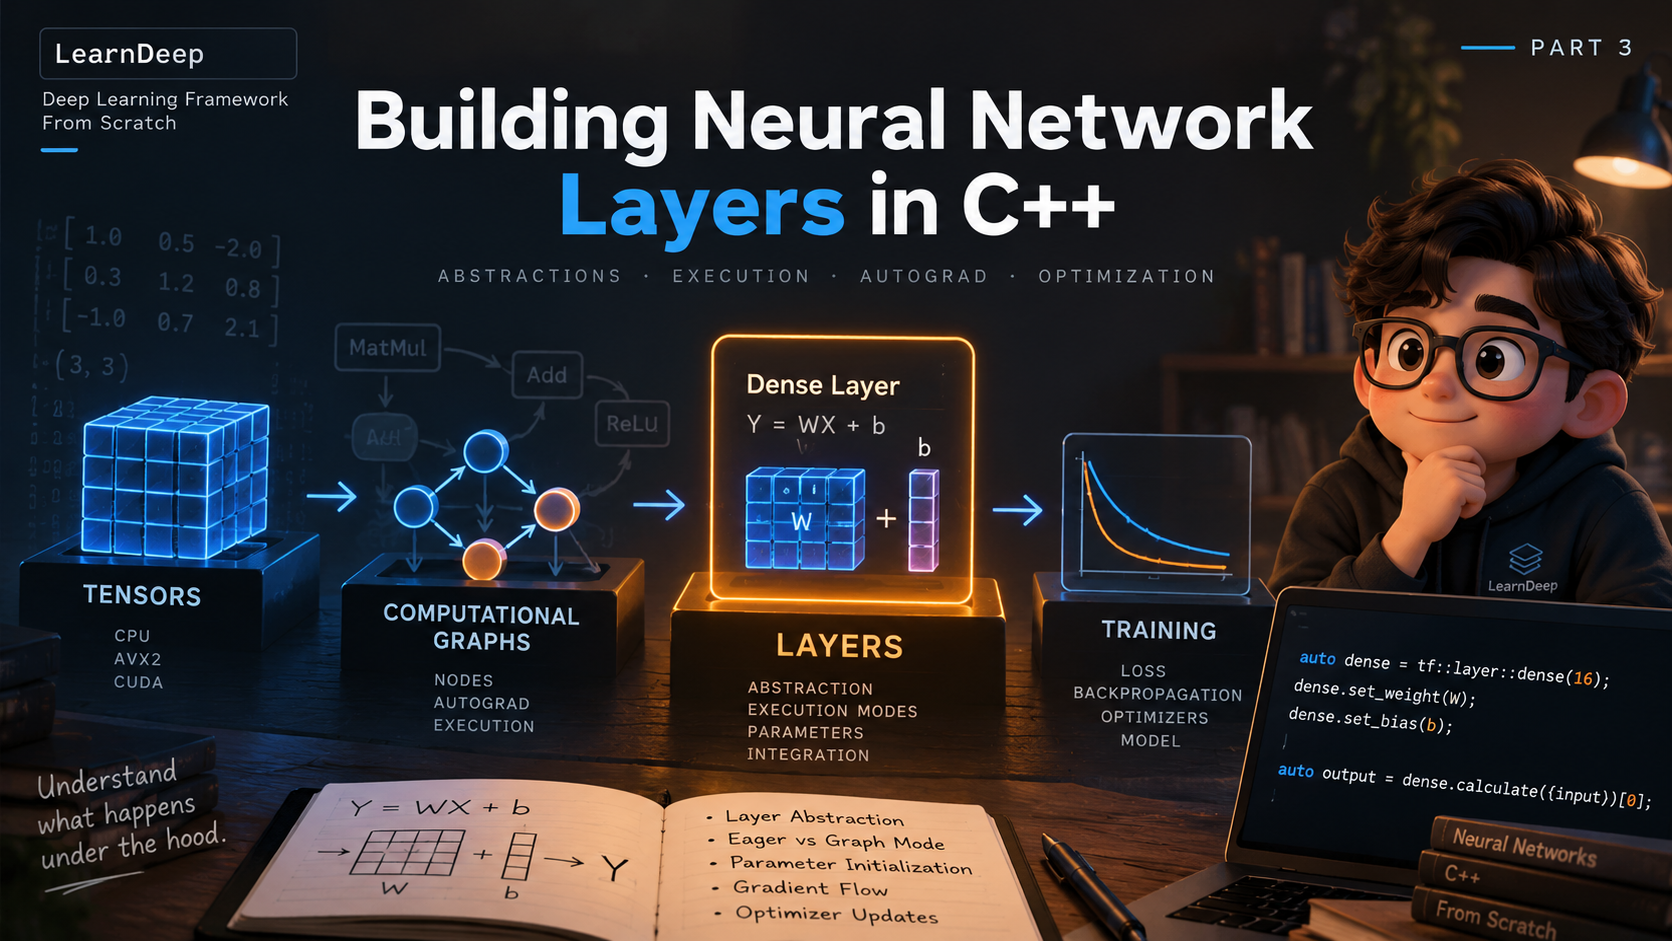
\includegraphics[width=\textwidth]{../../images/06_Building Neural Network Layers in C++.png
    }
\end{figure}

\section{Layer}
A layer is a high-level abstraction that encapsulates a
sequence of mathematical operations into a reusable
component. It allows us to construct complex neural
network architectures without explicitly writing
every underlying operation or manually defining the
backward graph for each layer.

This abstraction separates model architecture from the
mathematical details of individual operations. As a
result, we can modify the architecture and its
hyperparameters while relying on the framework to
handle the underlying computations and automatic
differentiation.

Let's now examine how layers are implemented in this framework.

The Layer class is an abstract base class that defines
the common interface for derived layers. Each concrete
layer implements the required functions:

the layer class is a abstruct class i.e can't be instantiated
then later layers are inheriting and overriding the functions
like
\begin{itemize}
    \item calculate: Calculates the forward pass only in eager
    mode
    \item forward: Constructs the layer's computation in the
    current graph context for graph-mode execution.
    \item backward: Retrieves the gradients required by the
    layer's parameters and registers the corresponding optimizer
    update operations. It does not explicitly construct the
    backward graph for the layer's mathematical operations;
    those gradients are handled by the autograd system.
    \item basic constructor and destructors and some axulary
    functions to intercept the parameters or hyperparameters.
\end{itemize}

Let's see it in practice

\begin{lstlisting}[
    caption={Creating layer class},
    label={lst:layer abstruct class}
]
class Layer {
public:
    virtual ~Layer() = default;

    virtual std::vector<tf::tensor>
    calculate(std::vector<tf::tensor> inputs) = 0;
    virtual std::vector<tf::tensor*>
    forward(std::vector<tf::tensor> inputs) = 0;
    virtual void backward() = 0;
};
\end{lstlisting}

Now lets take a look at each layer and how they're constructed

\section{Layer: Dense}

Mathematically Dense layer is very simple, it does matmul bias
add, which is

$
Y = X@W + b
$

\begin{itemize}
    \item X: input temsor of rank 2. axis-1 is feature
    axis-2 is batch or sample size.
    \item W: is weights tensor of rank 2 axis-1 is Dense
    unit/no or neuron axis-2 is no of incoming features.
    \item b: is a vector or matrix of rank 1. axis-1 is
    no of dense unit/ no of neuron.
    \item Y: output tensor of rank 2. axis-1 is no of
    feature and axis-2 is batch or sample size.
\end{itemize}

The idea behind Dense layer is do a linear transformation on
input with weights tensor and add bias to it.

If we wanted to implemente a dense layer without any layer
abstruction it would look something like


\begin{lstlisting}[
    caption={Dense Function},
    label={lst:Dense Function}
]
#include <tensor.h>

tf::tensor X, W, B, Y;

X.tf_create(18, 512); // no_of_input_feature(18), and sample_size(512)
W.tf_create(16, 18);  // dense_unit(16), and no_of_incoming_feature(18)
B.tf_create(18); // dense_unit(16);

Y = X.matmul(W).add(B);
\end{lstlisting}

First of all we can we that but if we think from bigger
perspective then it would be very clear that. This approch
is not that easy to scale. If we get to the training phase
then we need to mannually handle gradients and update them.
So that is the reason behind abstruction.

No Lets take a look at how to properly make the abstruction

\subsection{Dense: Constructor}

\begin{lstlisting}[
    caption={Dense constuctor and basic structure},
    label={lst:Dense constructor and basic structure}
]
// file dense.hpp
#include <layer.hpp>

Class Dense : protected Layer{
    Dense(unsigned unit): dense_unit(unit){}

    std::vector<tf::tensor *>& operator(std::vector<tf::tensor> input_tensors);
    std::vector<tf::tensor> calculate(std::vactor<tf::tensor> inputs) override;
    std::vector<tf::tensor *>& forward(std::vector<tf::tensor> inputs, unsigned const batch_size) override;
    std::vector<tf::tensor *>& backward(Optimizer *const optimizer) override;
    ...
    // few other internal methods/functions
    ...
}
\end{lstlisting}

simple easy peasy no rocket science. constructor
is expecting the no of neuron for this layer.
and assigning the vaue to its internal variable
and few other internal flags, weights, bias initialization
methods are set. Which is not shown here.

\subsection{Dense: Overloaded () operator}


\begin{lstlisting}[
    caption={Dense () overloaad},
    label={lst:Dense () overloaad}
]

// file dense.cpp
#include "dense.hpp"

const std::vector<tf::tensor *> &
Dense::operator()(std::vector<const tf::tensor> input_tensors){
    if(input_tensor.size() == 1){
        weights.tf_create();
        bias.tf_create();
        layer_outputs.push_back(tf::tensor(tf_float64));
    } else {
        // throw error, Dense layer expects only one input tensor
    }

}
\end{lstlisting}

The overloaded operator() provides a convenient
interface for connecting layers. During this
stage, the layer prepares its parameters and
output handles as required by the framework.

The initialization is lazy because the layer
may not have enough information to initialize
all its internal state when the constructor
is called. The first build or forward operation
provides the necessary context, such as the
input shape and batch size.

The output handle is particularly important:
it allows subsequent layers to reference the
output of this layer without manually
connecting every underlying mathematical
operation.

Why use vectors of tensors instead of a single
tensor? Although a Dense layer accepts one input
tensor and produces one output tensor, the base
interface supports layers that may consume
multiple inputs or produce multiple outputs.
This keeps the layer interface general without
forcing every layer to use the same input/output
cardinality.


\subsection{Dense: forward() backward() calculate()}

\begin{lstlisting}[
    caption={Dense calculate},
    label={lst:Dense calculate}
]

// file dense.cpp
#include "dense.hpp"

const std::vector<tf::tensor *> &
Dense::forward(std:;vector<const tf::tensor *> &inpyt, unsigned batch_size){

      this->weight.reshape(arr);
      this->training_weight.tf_create(arr, tf_float64);
      this->grad_weight.tf_create(arr, tf_float64);

      ...
      // initialize bias
      // initialize outputs
      ...

      training_output.push_back(training_input.matmul(training_weights).add(training_bias));

      return training_ouput;

}



const std::vector<tf::tensor *> &
Dense::calculate(std:;vector<const tf::tensor *> &inpyt, unsigned batch_size){
initializeParameters();
std::vector<tf::tensor> output;

output.emplace_back(inputs[0].matmul(weights).add(bias));

return output;
}

Dense::backward(Optimizer *optimizer){

  if (!this->isGradRecorded) {
    Graph *g = GraphManager::instance().getCurrentGraph();
    graph_weight = g->getGradTensor(training_weight);
    grad_bias =  g->getGradTensor(training_bias);
    grad_input = g->getGradTensor(training_inputs[0]);
    grad_output = g->getGradTensor(training_output[0]);

    optimizer->createParameterUpdateGraph(training_weight, updated_weight, grad_weight);
    optimizer->createParameterUpdateGraph(training_bias, updated_bias, grad_bias);

    this->isGradRecorded = true;
  }
}
\end{lstlisting}

Lets discuss one at a time:

\subsubsection{forward() }

This function implements the graph-mode forward
path and is primarily invoked during model
training through fit().

At this stage, the framework has access to the
execution context and the relevant input shapes.
The layer can initialize its parameters, prepare
the required tensors, and construct the
computation using the framework's primitive
operations.

The graph context is managed by the model's
training procedure, so the layer does not
need to create a separate graph context for
itself.

The important distinction is that forward()
constructs the computation graph; it does not
necessarily evaluate the tensor operations
immediately.

\subsubsection{calculate()}
This function implements the eager-mode
forward path and is primarily used by
predict() when immediate inference is
required.

Unlike graph construction, eager execution
evaluates the underlying operations as they
are invoked and returns the resulting
output tensors.

\subsubsection{backward()}
It retrieves the gradients associated with
the weights, biases, inputs, and outputs
from the current graph context, as required
by the implementation. It then registers
the parameter update operations with the
optimizer.

The gradients of the layer's mathematical
operations are computed by the autograd
system. The layer's backward() method
does not manually derive those gradients;
instead, it exposes the relevant gradient
tensors and prepares the optimizer update path.

The isGradRecorded flag prevents these
registrations from being repeated unnecessarily
within the intended graph lifecycle.

\subsection{Dense in practice}

\begin{lstlisting}[
    caption={Dense in practice},
    label={lst:Dense in practice}
]
// file dense_test_01.cpp
#include <tensor.h>

void main(){
    tf::tensor inputs, W, B, ouputs;

    inputs.tf_create(tf_float64, 19, 1000);
    W.tf_create(tf_float64, 16, 19); // tensor to seed weight
    B.tf_create(tf_tf_float64, 16);  // tensor to seed bias

    input.tensor_of(-2.0, 3.0);
    W.tensor_of(-1.0, 1.0);
    B.tensor_of(0.0, 0.0);

    auto dense = tf::layer::dense(16); // 16 is dense unit a.k.a no of neurons
    dense.set_weight(W);
    dense.set_bias(B);

    output = dense.calculate({inputs})[0]; // output holds the output from dense layer

}
\end{lstlisting}

\subsubsection{Dense Training}

backward(), is already covered so, we know
how it is done in code but let's touch upon
mathematical construct of Dense backward

Weight updation

\[ \bar{W} \leftarrow W - \nu * {\delta{W}} \]
\[ {\delta{W}} = ZX^T \]

Bias updation
\[ \bar{B} \leftarrow B - \nu * {\delta{B}} \]
\[ {\delta{W}} = X \]

Gradient propagation

\[ {\delta{X}} = W^TZ \]

The input gradient is propagated to the preceding
layer; it is not updated using the learning rate.
The optimizer updates trainable parameters, while
autograd propagates gradients through the
computational graph.


Where,
\[ Z \text{ is incoming grad} \]
\[ X \text{ is input} \]



\chapter{Neural Network Components: Losses}
\label{Losses}


\begin{figure}[!ht]
    \centering
    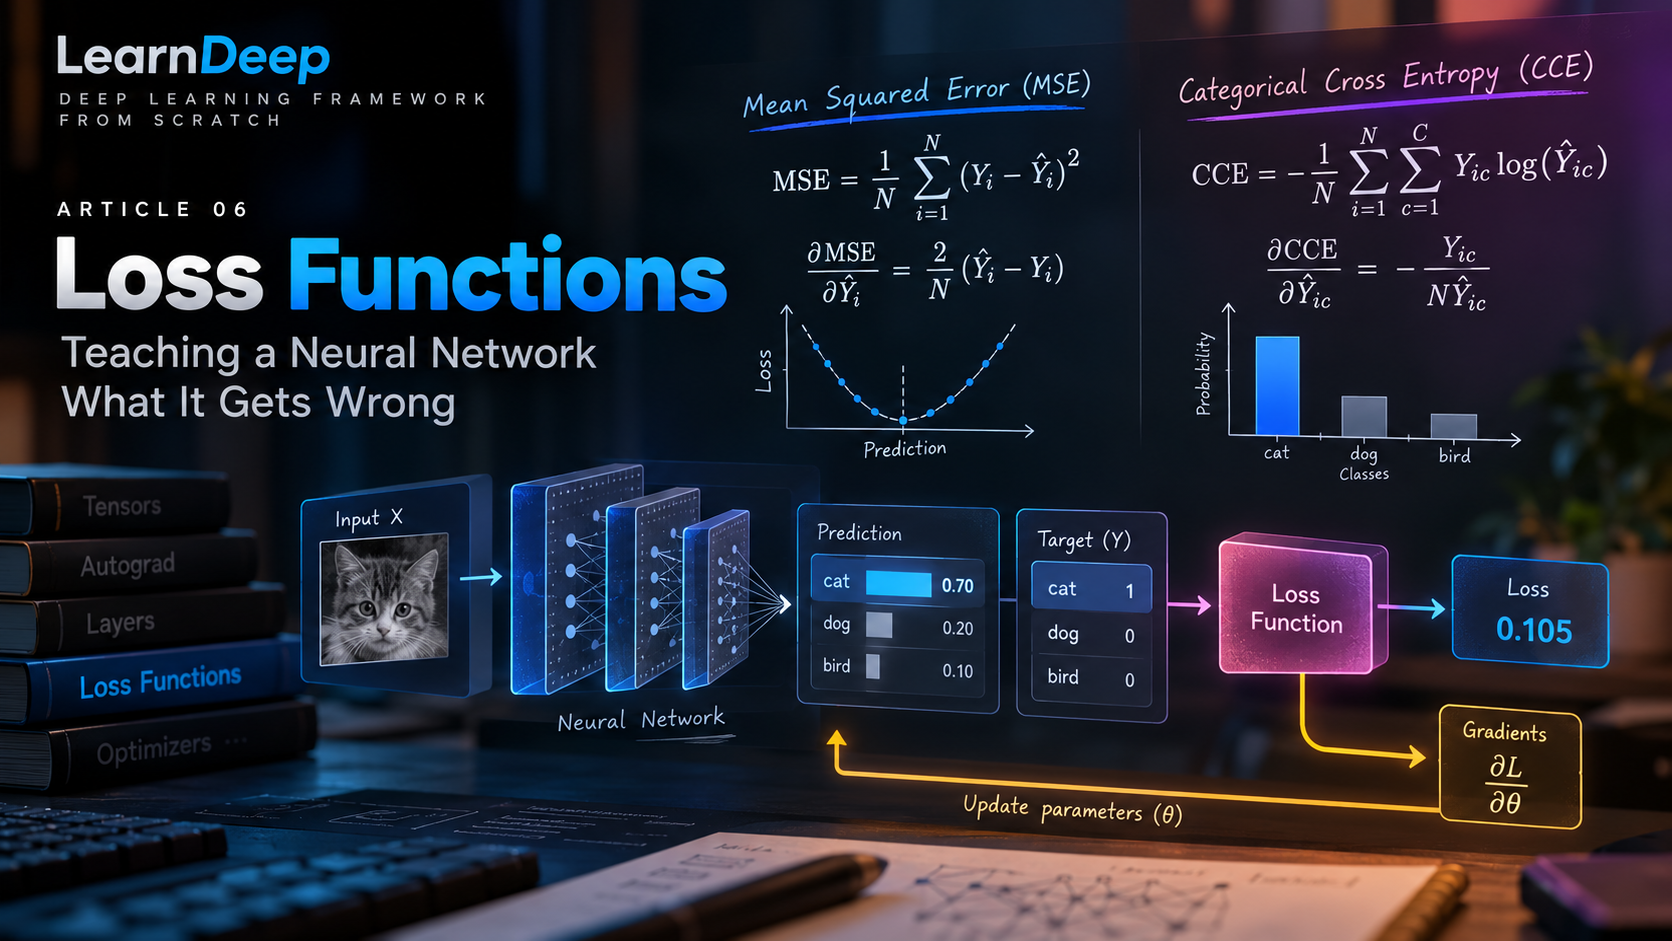
\includegraphics[width=\textwidth]{../../images/07_Neural Network Loss Functions Explained.png
    }
\end{figure}

% Document layers, loss functions, and model APIs here.

From the previous chapters, we've established
the core components of our framework, including
tensors, operations, autodiff, and neural
network components such as layers.

So far, our framework is good at performing
mathematical computations through forward and
backward passes. But how does it know whether
its predictions are correct? More importantly,
how does it know whether training is making
progress?

Our model's trainable parameters are initialized,
and gradients can be calculated through the
computational graph. But we still need a way
to measure the difference between the model's
predictions and the expected outputs.

That's where loss functions come in.

In supervised learning, a loss function measures
the discrepancy between predicted outputs and their
corresponding targets. During training, we typically
aim to minimize this loss. For each batch, the
model produces predictions during the forward pass,
and the loss function evaluates how far those
predictions are from the actual targets.

Let's see how this works in practice.

\section{Loss Functions: Mean Squared Error (MSE)}

\[
\mathrm{MSE} = \frac{1}{N}\sum_{i=1}^{N}(Y_i-\hat{Y}_i)^2
\]

where \(N\) is the number of elements over which
the squared errors are averaged, \(Y_i\) is the
target, and \(\hat{Y}_i\) is the predicted output.

For each element, we subtract the prediction from
the target and square the resulting difference. We
then calculate the mean of these squared errors
over the selected elements.

\subsection{MSE: Differentiation}

Although our autodiff engine calculates the gradients
automatically, let's look at the derivative to
understand what happens during backpropagation.

Differentiating MSE with respect to a prediction gives:

\[
\frac{\partial \mathrm{MSE}}{\partial \hat{Y}_i}
=\frac{2}{N}(\hat{Y}_i-Y_i)
\]

This gradient measures how the loss changes with
respect to each predicted value. Our autodiff
engine propagates it through the computational
graph to calculate gradients for the model's
trainable parameters.

\subsection{MSE: Putting things together}

Okey, now as we've sorted out the math part, we
can now focus on the implementation. If we think
deeply losses share common traits from their
bigger sibling layers. They have few differences

\begin{itemize}
    \item 1. Don't have trainable parameter
    \item 2. Outputs a scaler value rather than
    tensor.
\end{itemize}

So, we can follow same structure like Layers

\begin{lstlisting}[
    caption={Creating loss class},
    label={lst:layer abstruct class}
]
// file loss.hpp

class Loss {
public:
    virtual ~Loss() = default;

    virtual float calculate(std::vector<tf::tensor> inputs) = 0;
    virtual void forward(std::vector<tf::tensor> inputs) = 0;
    virtual void backward() = 0;
};
\end{lstlisting}

Although the loss function does not need to
implement differentiation manually, its backward
interface can provide access to the gradients
recorded by the computational graph. This is
useful for debugging and inspecting the
intermediate gradients.

Let's see how MeanSquaredError(MSE) is layed out.

\begin{lstlisting}[
    caption={Creating MSE class},
    label={lst:MSE class}
]
// file mse.cpp
#include <mse.hpp>

    void MSE::forward(std::vector<tf::tensor> inputs) {
      if (inputs.size() == 1) {
        training_inputs.push_back(inputs[0]);
        ...
        // initialize the intermediate tensors
        ...

        differences = target_ouput.sub(training_inputs[0]);
        loss_tensor = differences.pow(2).scale(1.0/batch_size);
      }
    };
    void MSE::backward(){
        if (!this->isGradRecorded) {
            this->isGradRecorded = true;
            Graph *g = GraphManager::instance().getCurrentGraph();
            grad_training_inputs = g,getGradTensor(trining_inputs[0]);
        }
    };
\end{lstlisting}

but sadly I've don't have any standalone
configuration to showcase how a user can
use losses. Most of its usage are inside
model. As of now simple eager execution is
not ready yet.

\section{Loss Function: Categorical Cross Entropy (CCE)}

While MSE is commonly used for regression tasks, Categorical Cross Entropy (CCE) is commonly used for classification tasks. It measures how well the predicted class probabilities match the target distribution.

For one-hot encoded targets, CCE is defined as:

\[
\mathrm{CCE}=-\frac{1}{N}
\sum_{i=1}^{N}\sum_{c=1}^{C}
Y_{ic}\log(\hat{Y}_{ic})
\]

where \(N\) is the batch size and \(C\) is the number of classes.

For each sample, we multiply the target value
for each class by the logarithm of its predicted
probability, sum over the classes, and average
over the batch. The negative sign ensures that
minimizing the loss encourages the model to
assign higher probabilities to the correct classes.

\subsection{CCE: Differentiation}

\[
\frac{\partial{CCE_\text{batch}}}{\partial{\hat(Y)}}= - \frac{1}{n}\frac{Y}{\hat{Y}}
\]

\subsection{CCE: Putting things together}

\begin{lstlisting}[
    caption={Creating CCE class},
    label={lst:CCE class}
]
// file cce.cpp
#include <cce.hpp>

    void CCE::forward(std::vector<tf::tensor> inputs) {
      if (inputs.size() == 1) {
        training_inputs.push_back(inputs[0]);
        ...
        // initialize the intermediate tensors
        ...

        log_differences = target_inputs[0].mul(training_inputs[0].log());
        loss_tensor = log_differences.scale(1.0/batch_size);
      }
    };
    void CCE::backward(){
        if (!this->isGradRecorded) {
            this->isGradRecorded = true;
            Graph *g = GraphManager::instance().getCurrentGraph();
            grad_training_inputs = g,getGradTensor(trining_inputs[0]);
        }
    };
\end{lstlisting}

\subsection{CCE: In practice}

Like MSE I've don't have eager mode calculate()
is still not ready. So I don't have much ex.
to showcase.

% Document layers, loss functions, and model APIs here.


\chapter{Neural Network Components: Optimizers}
\chapter{Neural Network Model Training and Inference}
\label{Model::Training}

\begin{figure}[!ht]
    \centering
    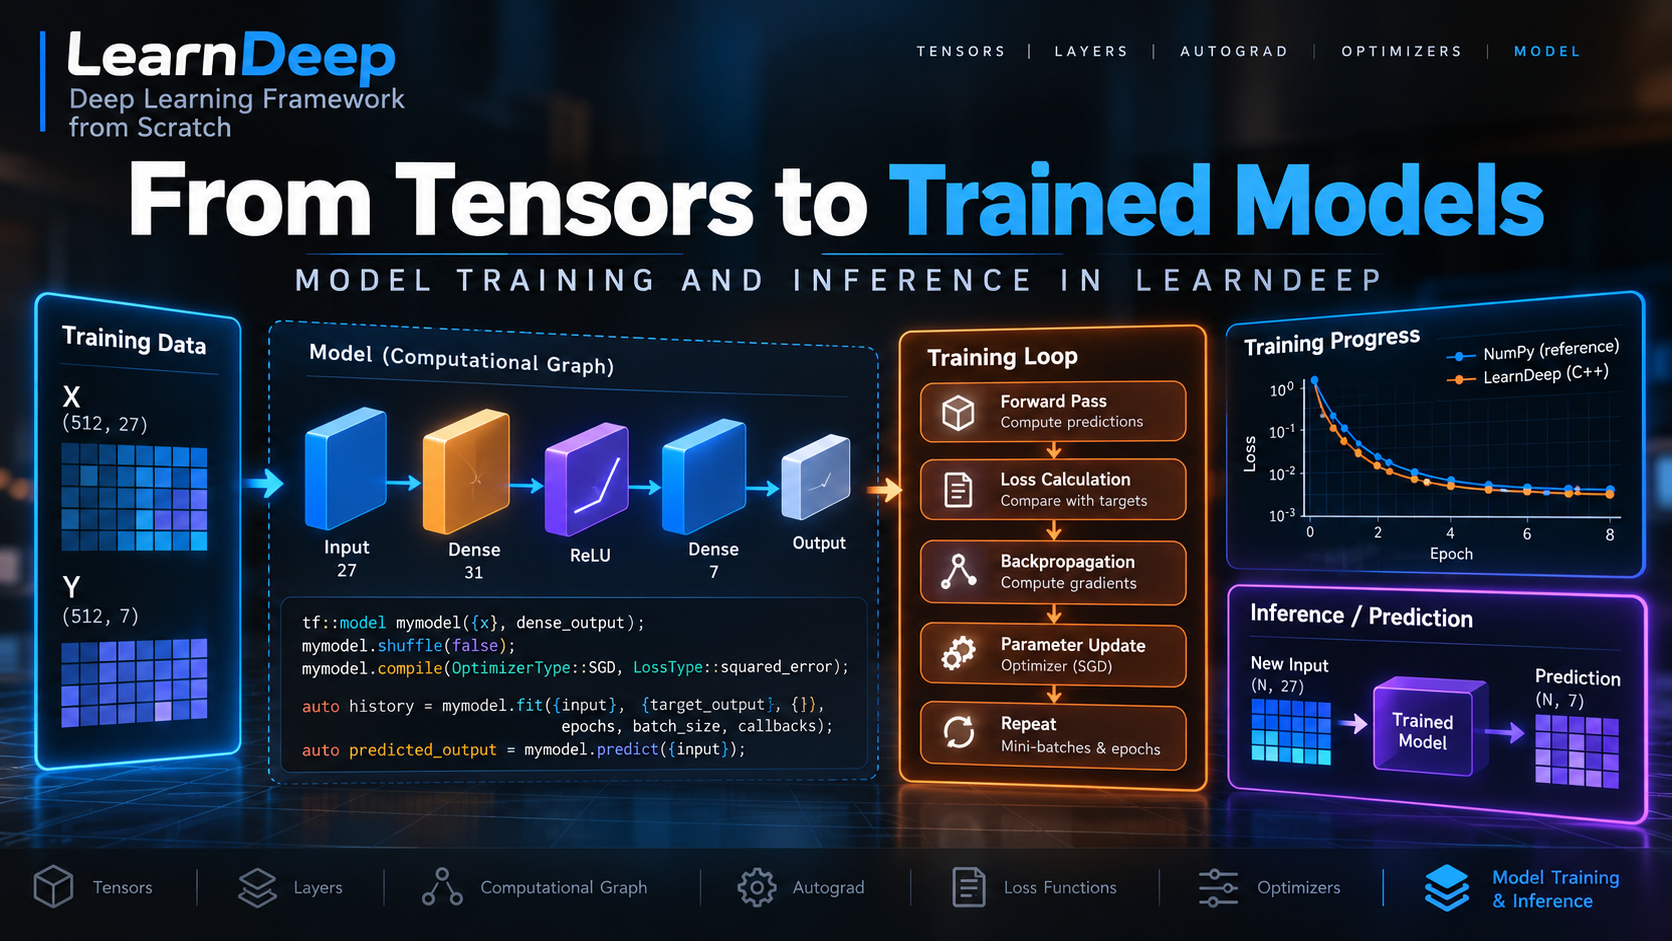
\includegraphics[width=\textwidth]{../../images/09_LearnDeep_ From Tensors to Trained Models.png
    }
\end{figure}

\paragraph{}
So far, we have developed the fundamental components required
to construct and train a neural network, including tensors,
layers, loss functions, optimizers, and automatic differentiation.

The next step is to bring these components together into a
complete training and inference workflow.

In this chapter, we will explore the public model API exposed
by LearnDeep and understand how it orchestrates the underlying
components. We will examine model construction, compilation,
training, and inference, and discuss how the implementation
can be verified against independently generated reference
results using NumPy.

The objective is not to revisit the implementation details of
each component, but to understand how they interact to form
a functional neural network framework.


\section{The Model Class}

The Model class provides the high-level interface through
which users define and execute a neural network. It abstracts
the underlying tensor operations, computational graph,
automatic differentiation, loss calculation, and parameter
optimization behind a small set of public API functions.

The following listing presents the principal interface of
the Model class.

\begin{lstlisting}[
    caption={Public interface of the Model class},
    label={lst:model_class}
]
class Model {
  void compile(const OptimizerType optimizer_type,
               const LossType loss_type);

  tf::history_container fit(
      const std::vector<tf::tensor>& inputs,
      const std::vector<tf::tensor>& outputs,
      const std::vector<tf::tensor>& validation_data = {},
      unsigned epochs = 10,
      unsigned batch_size = 1,
      std::vector<std::shared_ptr<Callback>> callback = {},
      unsigned verbose = 0,
      bool training = true);

  std::vector<tf::tensor> predict(
      std::vector<tf::tensor> inputs);

  void shuffle(bool shuffle);

  tf::loss getModelLoss(
      Tensor<std::float64_t>* output_tensor);
}
\end{lstlisting}

The API separates the definition of a model from the
operations performed on it. Model construction establishes
the relationship between input and output tensors, while
compilation configures the loss function and optimizer.
The fit() method coordinates training, and predict() provides
an interface for evaluating the model on new inputs.

The remaining methods support training configuration and
loss-related operations.

Let us examine how these responsibilities are implemented.


\subsection{Model Construction and Compilation}

Many neural network libraries provide a sequential interface
in which layers are arranged in a predefined order. Each layer
receives the output of the preceding layer and passes its own
output to the next layer.

LearnDeep instead represents a model through its input and
output tensors and the computational dependencies connecting
them. This approach is not restricted to a sequential
arrangement of layers.

For example, consider the following model construction:

\begin{lstlisting}[
    caption={Constructing and compiling a model},
    label={lst:model construction}
]
tf::model mymodel({x}, dense_output);

mymodel.shuffle(false);

mymodel.compile(OptimizerType::SGD,
                LossType::squared_error);
\end{lstlisting}

Here, x represents the model input, while dense\_output
represents the output tensor produced by the network.
The model is constructed by associating these tensors,
rather than by explicitly passing an ordered collection
of layers to the Model constructor.

During model construction, LearnDeep traverses the
dependencies of the declared output tensors to determine
whether they can be traced back to the declared inputs.
If the required dependencies cannot be resolved, the
model construction is rejected.

This process establishes the computational path required
to evaluate the model. It also provides the foundation
for executing the forward computation and, during training,
propagating gradients through the relevant operations.

The distinction between a sequential arrangement and
a computational graph becomes particularly important
when a model contains multiple inputs, branching paths,
or operations that combine outputs from different parts
of the network.

The supported graph structures ultimately depend on the
operations and execution strategies implemented by
LearnDeep.

\paragraph{Compilation}

Once the model has been constructed, compile() configures
the components required for training.

The optimizer type determines the parameter update strategy,
while the loss type determines how the model's predictions
are evaluated against the target outputs.

For example, the configuration shown above selects
stochastic gradient descent (SGD) as the optimizer and
squared error as the loss function.

Based on these selections, LearnDeep creates the corresponding
optimizer and loss instances. This separates the choice of
training configuration from the implementation of the
training loop itself.

The optimizer and loss function serve different purposes.
The loss function quantifies the prediction error, whereas
the optimizer uses the resulting gradients to update the
trainable parameters.

\paragraph{Training Data Shuffling}

The shuffle() method controls whether the training samples
are shuffled before being divided into mini-batches.

When shuffling is disabled, the samples retain their original
order. When enabled, their order is randomized according to
the implementation.

In the example above, shuffle(false) preserves the original
sample order.

Shuffling is useful during training because it reduces
dependence on the original ordering of the training samples.
However, it does not change the underlying model architecture
or the mathematical definition of its operations.


\subsection{Model Training}

Training is the process through which a neural network
adjusts its trainable parameters to reduce the discrepancy
between its predictions and the target outputs.

The fit() method provides the interface for executing this
process.

\begin{lstlisting}[
    caption={Training a model},
    label={lst:model_training}
]
unsigned epochs = 10;
unsigned batch_size = 128;

auto history = mymodel.fit(
    {input},
    {target_output},
    {},
    epochs,
    batch_size,
    callback);
\end{lstlisting}

The training inputs and corresponding target outputs are
provided as collections of tensors. The epochs argument
specifies how many complete passes are performed over the
training dataset, while batch\_size determines the number
of samples processed in an individual mini-batch.

During training, the framework coordinates the following
operations:

\begin{enumerate}
    \item \textbf{Mini-batch selection:}
    The training samples are divided into batches according
    to the configured batch size and shuffling policy.

    \item \textbf{Forward propagation:}
    The input tensors are passed through the computational
    graph to calculate the model predictions.

    \item \textbf{Loss calculation:}
    The predictions are compared with the corresponding
    target outputs using the configured loss function.

    \item \textbf{Backward propagation:}
    Automatic differentiation computes the gradients of
    the loss with respect to the trainable parameters.

    \item \textbf{Parameter optimization:}
    The optimizer uses the calculated gradients to update
    the model parameters.

    \item \textbf{Iteration:}
    The process continues for the remaining mini-batches
    and repeats until the requested number of epochs
    has been completed.
\end{enumerate}

The process connects the components developed in the
previous chapters. Tensor operations perform the forward
computation, the loss function evaluates the predictions,
automatic differentiation calculates gradients, and the
optimizer updates the parameters.

The fit() method therefore acts as the coordinator of
the training workflow rather than implementing each of
these operations independently.

\paragraph{Callbacks and Training History}

Callbacks provide a mechanism for observing or responding
to events during training. Depending on the callback
implementation, they can be used to record metrics,
monitor training progress, or control the training process.

The fit() method returns a history container that preserves
the training information recorded during execution.
This allows the user to inspect the training results
after the fit() call has completed.

The exact contents of the history depend on the metrics
and callback behavior supported by LearnDeep.

The validation data argument can be used to provide
additional data for evaluating the model during training,
provided that validation evaluation is implemented by
the training workflow. Validation data is distinct from
the training data because it is used to evaluate model
behavior rather than to perform gradient-based parameter
updates.


\subsection{Model Inference}

After training, the model can be used to generate
predictions for a given set of input tensors.

Inference evaluates the model using its current parameter
values without performing optimizer-driven parameter
updates.

The predict() method provides this interface.

\begin{lstlisting}[
    caption={Generating predictions using a trained model},
    label={lst:model_inference}
]
auto predicted_output = mymodel.predict({input});
\end{lstlisting}

The input tensors are evaluated through the model's
computational graph, and the resulting output tensors
are returned to the caller.

Unlike training, inference does not require target outputs
or a loss calculation for the purpose of updating model
parameters. Its primary responsibility is to produce
predictions from the supplied inputs.

When predict() is called on a model that has already
been trained, it uses the model's current weights and
biases. Consequently, the predictions reflect the
parameter updates performed during training.

Separating training from inference provides a clear
distinction between learning the model parameters and
using those parameters to evaluate new data.


\section{Numerical Verification}

Implementing the model API is only one part of developing
a neural network framework. Its numerical behavior must
also be verified against a trusted reference.

LearnDeep uses NumPy to generate reference results for
selected operations and model configurations. These
results can then be compared against the outputs produced
by the C++ implementation.

For a forward-pass test, the model is configured with
known weights and biases, and its predictions are compared
with the corresponding NumPy results. This helps verify
that the model correctly combines its underlying tensor
operations.

Training requires additional verification. The parameter
updates and loss behavior should be examined independently
to establish that gradients and optimization are working
as intended.

Finally, inference can be tested by checking whether
predict() returns the expected output tensors for a known
model state and a given set of inputs.

These tests address different aspects of correctness:
forward-pass tests verify numerical computation, training
tests examine gradient-based optimization, and inference
tests verify the prediction interface.

Together, they provide a systematic approach to validating
the integration of the components developed throughout
this framework.

\[
\nabla_\theta L
\]

% Document training loops, optimizers, callbacks,
% and prediction here.

\end{document}